%%%%%%%%%%%%%%%%%%%%%%%%%%%%%%%%%%%%%%%%%
% Structured General Purpose Assignment
% LaTeX Template
%
% This template has been downloaded from:
% http://www.latextemplates.com
%
% Original author:
% Ted Pavlic (http://www.tedpavlic.com)
%
% Note:
% The \lipsum[#] commands throughout this template generate dummy text
% to fill the template out. These commands should all be removed when 
% writing assignment content.
%
%%%%%%%%%%%%%%%%%%%%%%%%%%%%%%%%%%%%%%%%%

%----------------------------------------------------------------------------------------
%	PACKAGES AND OTHER DOCUMENT CONFIGURATIONS
%----------------------------------------------------------------------------------------

\documentclass{article}

\usepackage{fancyhdr} % Required for custom headers
\usepackage{lastpage} % Required to determine the last page for the footer
\usepackage{extramarks} % Required for headers and footers
\usepackage{graphicx} % Required to insert images
\usepackage{lipsum} % Used for inserting dummy 'Lorem ipsum' text into the template
\usepackage{listings}
\usepackage{color}
\usepackage{amsmath}

\definecolor{dkgreen}{rgb}{0,0.6,0}
\definecolor{gray}{rgb}{0.5,0.5,0.5}
\definecolor{mauve}{rgb}{0.58,0,0.82}

\lstset{frame=tb,
  language=R,
  aboveskip=3mm,
  belowskip=3mm,
  showstringspaces=false,
  columns=flexible,
  basicstyle={\small\ttfamily},
  numbers=none,
  numberstyle=\tiny\color{gray},
  keywordstyle=\color{blue},
  commentstyle=\color{dkgreen},
  stringstyle=\color{mauve},
  breaklines=true,
  breakatwhitespace=true
  tabsize=3
}

% Margins
\topmargin=-0.45in
\evensidemargin=0in
\oddsidemargin=0in
\textwidth=6.5in
\textheight=9.0in
\headsep=0.25in 

\linespread{1.1} % Line spacing

% Set up the header and footer
\pagestyle{fancy}
\lhead{\hmwkAuthorName} % Top left header
\chead{\hmwkClass\ (\hmwkClassInstructor\ \hmwkClassTime): \hmwkTitle} % Top center header
\rhead{\firstxmark} % Top right header
\lfoot{\lastxmark} % Bottom left footer
\cfoot{} % Bottom center footer
\rfoot{Page\ \thepage\ of\ \pageref{LastPage}} % Bottom right footer
\renewcommand\headrulewidth{0.4pt} % Size of the header rule
\renewcommand\footrulewidth{0.4pt} % Size of the footer rule

\setlength\parindent{0pt} % Removes all indentation from paragraphs

%----------------------------------------------------------------------------------------
%	DOCUMENT STRUCTURE COMMANDS
%	Skip this unless you know what you're doing
%----------------------------------------------------------------------------------------

% Header and footer for when a page split occurs within a problem environment
\newcommand{\enterProblemHeader}[1]{
\nobreak\extramarks{#1}{#1 continued on next page\ldots}\nobreak
\nobreak\extramarks{#1 (continued)}{#1 continued on next page\ldots}\nobreak
}

% Header and footer for when a page split occurs between problem environments
\newcommand{\exitProblemHeader}[1]{
\nobreak\extramarks{#1 (continued)}{#1 continued on next page\ldots}\nobreak
\nobreak\extramarks{#1}{}\nobreak
}

\setcounter{secnumdepth}{0} % Removes default section numbers
\newcounter{homeworkProblemCounter} % Creates a counter to keep track of the number of problems

\newcommand{\homeworkProblemName}{}
\newenvironment{homeworkProblem}[1][Problem \arabic{homeworkProblemCounter}]{ % Makes a new environment called homeworkProblem which takes 1 argument (custom name) but the default is "Problem #"
\stepcounter{homeworkProblemCounter} % Increase counter for number of problems
\renewcommand{\homeworkProblemName}{#1} % Assign \homeworkProblemName the name of the problem
\section{\homeworkProblemName} % Make a section in the document with the custom problem count
\enterProblemHeader{\homeworkProblemName} % Header and footer within the environment
}{
\exitProblemHeader{\homeworkProblemName} % Header and footer after the environment
}

\newcommand{\problemAnswer}[1]{ % Defines the problem answer command with the content as the only argument
\noindent\framebox[\columnwidth][c]{\begin{minipage}{0.98\columnwidth}#1\end{minipage}} % Makes the box around the problem answer and puts the content inside
}

\newcommand{\homeworkSectionName}{}
\newenvironment{homeworkSection}[1]{ % New environment for sections within homework problems, takes 1 argument - the name of the section
\renewcommand{\homeworkSectionName}{#1} % Assign \homeworkSectionName to the name of the section from the environment argument
\subsection{\homeworkSectionName} % Make a subsection with the custom name of the subsection
\enterProblemHeader{\homeworkProblemName\ [\homeworkSectionName]} % Header and footer within the environment
}{
\enterProblemHeader{\homeworkProblemName} % Header and footer after the environment
}
   
%----------------------------------------------------------------------------------------
%	NAME AND CLASS SECTION
%----------------------------------------------------------------------------------------

\newcommand{\hmwkTitle}{Quiz\ \#1} % Assignment title
\newcommand{\hmwkDueDate}{July 15,\ 2014} % Due date
\newcommand{\hmwkClass}{Advanced Calculus} % Course/class
\newcommand{\hmwkClassTime}{6:00 pm} % Class/lecture time
\newcommand{\hmwkClassInstructor}{Dan Stefanica} % Teacher/lecturer
\newcommand{\hmwkAuthorName}{Weiyi Chen} % Your name

%----------------------------------------------------------------------------------------
%	TITLE PAGE
%----------------------------------------------------------------------------------------

\title{
\vspace{2in}
\textmd{\textbf{\hmwkClass:\ \hmwkTitle}}\\
\normalsize\vspace{0.1in}\small{Due\ on\ \hmwkDueDate}\\
\vspace{0.1in}\large{\textit{\hmwkClassInstructor\ \hmwkClassTime}}
\vspace{3in}
}

\author{\textbf{\hmwkAuthorName}}
\date{} % Insert date here if you want it to appear below your name

%----------------------------------------------------------------------------------------

\begin{document}

\maketitle

%----------------------------------------------------------------------------------------
%	TABLE OF CONTENTS
%----------------------------------------------------------------------------------------

%\setcounter{tocdepth}{1} % Uncomment this line if you don't want subsections listed in the ToC

%\newpage
%\tableofcontents
\newpage

%----------------------------------------------------------------------------------------
%	PROBLEM 1
%----------------------------------------------------------------------------------------

\begin{homeworkProblem}
  Compute
  \begin{equation}
    \lim_{x\to\infty}3x^2-\sqrt{9x^4+12x^2+7}
  \end{equation}
  \begin{homeworkSection}{Answer}
  \begin{equation}
    \begin{split}
      \lim_{x\to\infty}3x^2-\sqrt{9x^4+12x^2+7} &= \lim_{x\to\infty} \frac{(3x^2-\sqrt{9x^4+12x^2+7})(3x^2+\sqrt{9x^4+12x^2+7})}{3x^2+\sqrt{9x^4+12x^2+7}} \\
      &= \lim_{x\to\infty} \frac{(3x^2)^2 - (\sqrt{9x^4+12x^2+7})^2}{3x^2+\sqrt{9x^4+12x^2+7}} \\
      &= \lim_{x\to\infty} \frac{-12x^2-7}{3x^2+\sqrt{9x^4+12x^2+7}} \\
      &= \lim_{x\to\infty} \frac{-12-\frac{7}{x^2}}{3+\sqrt{9+\frac{12}{x^2}+\frac{7}{x^4}}} \\
      &= \frac{-12}{3+\sqrt{9}} \\
      &= -2
    \end{split}
  \end{equation}
  \end{homeworkSection}
\end{homeworkProblem}


%----------------------------------------------------------------------------------------
% PROBLEM 2
%----------------------------------------------------------------------------------------
\newpage
\begin{homeworkProblem}
Compute
\begin{equation}
  \begin{split}
    &\frac{\partial}{\partial x}(\frac{1}{1+tx})^n \\
    &\frac{\partial}{\partial x_{j}} (\prod_{i=1}^{n} \frac{1}{1+tx_i})
  \end{split}
\end{equation}
\begin{homeworkSection}{Answer}
  \begin{equation}
    \begin{split}
      \frac{\partial}{\partial x}(\frac{1}{1+tx})^n &= \frac{\partial}{\partial x}(1+tx)^{-n} \\
      &= (-n)(1+tx)^{-n-1} \frac{\partial}{\partial x}(1+tx) \\
      &= -nt(1+tx)^{-n-1}
    \end{split}
  \end{equation}
  \begin{equation}
    \begin{split}
      \frac{\partial}{\partial x_{j}} (\prod_{i=1}^{n} \frac{1}{1+tx_i}) &= (\prod_{i\neq j} \frac{1}{1+tx_i}) \frac{\partial}{\partial x_{j}} (\frac{1}{1+tx_j}) \\
      &= (\prod_{i\neq j} \frac{1}{1+tx_i}) (-t(1+tx_j)^{-2}) \\
      &= -\frac{t}{1+tx_j} (\prod_{i=1}^{n} \frac{1}{1+tx_i})
    \end{split}
  \end{equation}
\end{homeworkSection}
\end{homeworkProblem}

%----------------------------------------------------------------------------------------
% PROBLEM 3
%----------------------------------------------------------------------------------------
\newpage
\begin{homeworkProblem}
Compute
\begin{equation}
  \lim_{x\to0} \frac{N(x)-\frac{1}{2}-\frac{x}{\sqrt{2\pi}}}{x^3}
\end{equation}
where
\begin{equation}
  N(x) = \frac{1}{\sqrt{2\pi}} \int_{-\infty}^{x}e^{-y^2/2}dy
\end{equation}
is the cumulative density function of the standard normal variable.
\begin{homeworkSection}{Answer}
  Since
  \begin{equation}
    \lim_{x\to0} N(x)-\frac{1}{2}-\frac{x}{\sqrt{2\pi}} = 0
  \end{equation}
  and 
  \begin{equation}
    \lim_{x\to0} x^3 = 0
  \end{equation}
  We can use l'Hospital's rule, that is
  \begin{equation}
    \begin{split}
      \lim_{x\to0} \frac{N(x)-\frac{1}{2}-\frac{x}{\sqrt{2\pi}}}{x^3} &= \lim_{x\to0} \frac{N'(x)-\frac{1}{\sqrt{2\pi}}}{3x^2} \\
      &= \frac{1}{3\sqrt{2\pi}} \lim_{x\to0} \frac{e^{x^2/2} - 1}{x^2}
    \end{split}
  \end{equation}
  where 
  \begin{equation}
    N'(x) = \frac{1}{\sqrt{2\pi}} e^{-x^2/2}
  \end{equation}
  Similarly, using l'Hospital's rule,
    \begin{equation}
    \begin{split}
      \frac{1}{3\sqrt{2\pi}} \lim_{x\to0} \frac{e^{x^2/2} - 1}{x^2} &= \frac{1}{3\sqrt{2\pi}} \lim_{x\to0} \frac{e^{-x^2/2}(-x)}{2x} \\
      &= -\frac{1}{6\sqrt{2\pi}} \lim_{x\to0} e^{-x^2/2} \\
      &= -\frac{1}{6\sqrt{2\pi}}
    \end{split}
  \end{equation}
\end{homeworkSection}
\end{homeworkProblem}

%----------------------------------------------------------------------------------------
% PROBLEM 4
%----------------------------------------------------------------------------------------
\newpage
\begin{homeworkProblem}
(i) Synthesize a long position in a 36–42 bull spread using the 36 strike and the 42 strike put options. Draw the payoff diagram and the P\&L diagram at maturity of this position. For what values of the underlying asset at maturity does the position make money? \\
(ii) Synthesize a long position in a 36–42 bull spread using the 36 strike and the 42 strike call options. Draw the payoff diagram and the P\&L diagram at maturity of this position. For what values of the underlying asset at maturity does the position make money?\\
\begin{homeworkSection}{(i)}
  A long position in a 36–42 bull spread can be synthesized by long the 36 strike put options and short the 42 strike put options. The payoff of the bull spread is \\
  \begin{equation}
    \begin{split}
      V(T) &= \max(36-S(T),0) - \max(42-S(T),0) \\
      &= 
      \begin{cases}
        -6, & \text{if } S(T)<36 \\
        S(T)-42, & \text{if } 36\le S(T) < 42 \\
        0, & \text{if } 42 \le S(T)
      \end{cases}
    \end{split}
  \end{equation}
  The P\&L at maturity of this position is \\ 
  \begin{equation}
    \begin{split}
      P\&L(T) &= V(T)+4-1.2 \\
      &= 
      \begin{cases}
        -3.2, & \text{if } S(T)<36 \\
        S(T)-39.2, & \text{if } 36\le S(T) < 42 \\
        2.8, & \text{if } 42 \le S(T)
      \end{cases}
    \end{split}
  \end{equation}
  The payoff diagram and the P\&L diagram at maturity of this position is
  \begin{figure*}[ht]\centering
    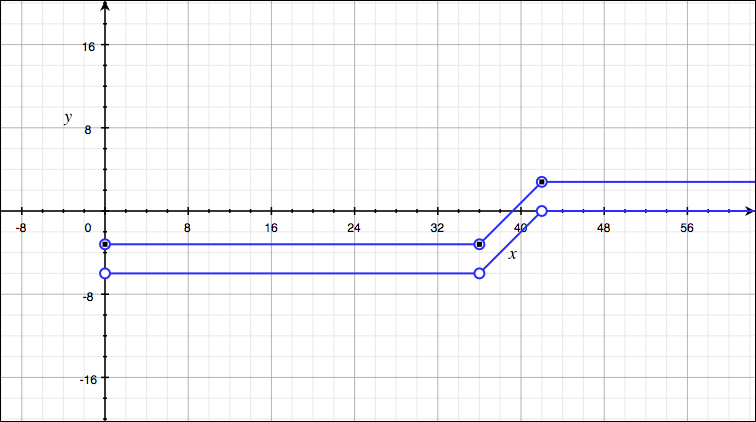
\includegraphics[scale=0.5]{ps4}
  \end{figure*}
  \\ where the hollow points represent payoff and the solid points represent P\&L. \\
  For the underlying asset at maturity with $S(T) > 39.2$, the position makes money.
\end{homeworkSection}
\newpage
\begin{homeworkSection}{(ii)}
  A long position in a 36–42 bull spread can be synthesized by long the 36 strike call options and short the 42 strike call options. The payoff of the bull spread is \\
  \begin{equation}
    \begin{split}
      V(T) &= \max(S(T)-36,0) - \max(S(T)-42,0) \\
      &= 
      \begin{cases}
        0, & \text{if } S(T)<36 \\
        S(T)-36, & \text{if } 36\le S(T) < 42 \\
        6, & \text{if } 42 \le S(T)
      \end{cases}
    \end{split}
  \end{equation}
  The P\&L at maturity of this position is \\ 
  \begin{equation}
    \begin{split}
      P\&L(T) &= V(T)+5.5-2.5 \\
      &= 
      \begin{cases}
        -3, & \text{if } S(T)<36 \\
        S(T)-39, & \text{if } 36\le S(T) < 42 \\
        3, & \text{if } 42 \le S(T)
      \end{cases}
    \end{split}
  \end{equation}
  The payoff diagram and the P\&L diagram at maturity of this position is
  \begin{figure*}[ht]\centering
    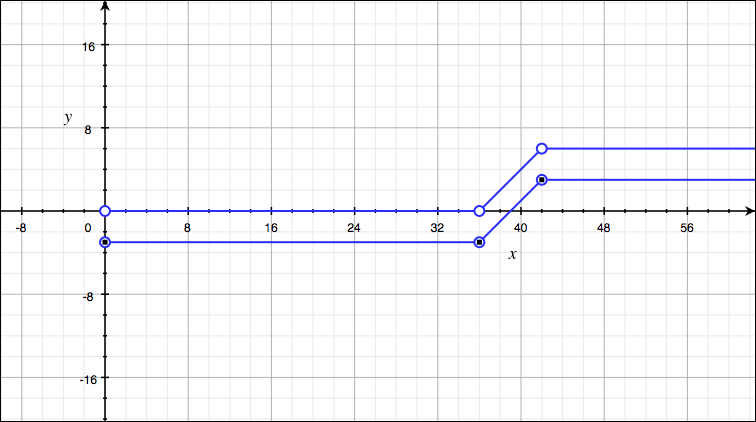
\includegraphics[scale=0.5]{ps5}
  \end{figure*}
  \\ where the hollow points represent payoff and the solid points represent P\&L. \\
  For the underlying asset at maturity with $S(T) > 39$, the position makes money.
\end{homeworkSection}
\end{homeworkProblem}

%----------------------------------------------------------------------------------------
% PROBLEM 5
%----------------------------------------------------------------------------------------
\newpage
\begin{homeworkProblem}
 The bid and ask prices for nine months ATM European options on an underlying asset paying 1\% dividends continuously and with spot price \$60 are
 \begin{equation}
   \begin{split}
    &C_{bid} = 6; C_{ask} = 6.5; \\
    &P_{bid} = 5.5; P_{ask} = 6.
   \end{split}
 \end{equation}
\begin{homeworkSection}{Answer}
  According to the put-call parity, an arbitrage exists if 
  \begin{equation}
    C_{bid} - P_{ask} > Se^{-qT} - Ke^{-rT}
  \end{equation}
  or
  \begin{equation}
    C_{ask} - P_{bid} < Se^{-qT} - Ke^{rT}
  \end{equation}
  However we find that
  \begin{equation}
    \begin{split}
      C_{bid} - P_{ask} &= 6 - 6 = 0 \\
      C_{ask} - P_{bid} &= 6.5 - 5.5 = 1 \\
      Se^{-qT} - Ke^{-rT} &= 60(e^{-0.01\times0.75}-e^{-0.01\times0.75})= 0.887 \in [0,1]
    \end{split}
  \end{equation}
  Therefore there is no arbitrage opportunity present.
\end{homeworkSection}
\end{homeworkProblem}

\end{document}